\documentclass[10pt,a4paper]{article}
\usepackage[utf8]{inputenc}
\usepackage{amsmath}
\usepackage{amsfonts}
\usepackage{amssymb}
\usepackage{eucal}
\usepackage{physics}
\usepackage{graphicx}

\begin{document}

\section{Introduction}

Quantum computing has meant a paradigm shift in computer science, introducing a new era of computational power and possibilities. By leveraging the principles of quantum mechanics, quantum computing offers capabilities far beyond those of classical computers. Although quantum hardware is still evolving, Noisy Intermediate-Scale Quantum (NISQ) \cite{Preskill} computers have already begun to unveil the potential of quantum computing, igniting widespread interest in implementing quantum algorithms that promise significant speedups over classical counterparts. In particular, the speedup of solving NP-complete problems is an area that quantum computing can tackle. In this paper, we have focused on the Hamiltonian Cycle Problem.In this paper, we propose utilizing Grover's algorithm to tackle the HC problem, offering the potential for quadratic speedup.\\
The structure of this paper is as follows. An explanation of Grover's algorithm and background on the HC problem are given in Section II. The proposed methodology is given in Section III. Section IV generalizes the proposed solution and reduces the quantity of qubits necessary. Section V provides a discussion on the algorithm's implementation and complexity. Finally, Section VI concludes the paper and suggests future work.\\


\section{Background}
\subsection{Grover's Algorithm}

The search algorithm developed by Lov K. Grover in 1997 \cite{Grover1} is a milestone in the development of quantum algorithms. It solves the problem of finding a tagged element (or $M$ elements) in a disordered set of $N$ elements using $k_{Gr}= \left\lfloor\frac{\pi}{4} \sqrt{\frac{N}{M}}\right\rfloor$ times a system, called oracle, which is able to identify this element. It presents a quadratic improvement in order relative to the classical brute-force search algorithm, which requires in the worst-case scenario N system calls. Grover's algorithm does not converge with 100\% probability to the desired state, it converges with an arbitrarily high probability that depends on the relationship between solutions and the size of the search space.\\
As Grover proposed later, the algorithm can be used to speed up the solution of NP-complete problems \cite{Grover2}. Since, its application has been explored with some problems such as Clique problem \cite{Clique, Clique2}, k-coloring \cite{Coloring1, Coloring2} and SAT \cite{SAT_ions, SAT_paralel}. Nielsen and Chuang predicted the solution of the HC problem using Grover\cite{Nielsen_Chuang_2010}.\\
The original problem presented by Grover \cite{Grover1} is as follows. Let there be a set of $N = 2^n$ quantum states in a Hilbert space ($\mathcal{H}_n$), where n is the number of qubits, and an unknown canonical basis state marked between them (solution to the problem). Given an oracle that identifies the marked element, the objective is to find this marked element with high probability, using as few queries to the oracle as possible.\\
Let $\ket{t}$ be the marked element of the base, and $\ket{s}$ the uniform superposition of all basis states. An oracle operator $O = I_d - 2\ket{t}\bra{t}$ is applied and changes the phase of the marked state. A diffusion operator $D = I_d - 2\ket{s}\bra{s}$ is applied and amplifies the amplitude of the marked state. Applying the Grover operator $(G=DO)$ $k_{Gr}$ times maximizes the probability of measuring $\ket{t}$.\\
A more detailed and extended explanation for when the set has more than one solution can be found in reference \cite{Nielsen_Chuang_2010}.

\begin{figure}[hbtp]
\centering
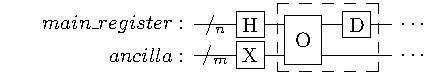
\includegraphics[scale=1.5]{figures/grover.pdf}
\caption{Grover's algorithm circuit, the Grover operator $G = DO$ is applied $k_{Gr}$ times.}
\end{figure}

\subsection{Hamiltonian Cycle Problem}
A Hamiltonian cycle in a graph is a closed loop that visits every vertex exactly once, returning to the starting vertex. Formally, given a graph $G = (V, E)$, a Hamiltonian cycle is a permutation of the vertices $(v_1, v_2, ..., v_n)$ such that for each $i$ from $1$ to $n-1$, there exists an edge $\{v_i, v_{i+1}\}$ in $E$, and there is also an edge $\{v_n, v_1\}$ in $E$, completing the cycle.\\
This problem is one of Karp's 21 seminal NP-complete problems \cite{Karp1972}, it involves determining whether a given graph contains a cycle that visits every vertex exactly once. The problem is significant because of its similarities with the TSP, and its applications span various domains, including logistics and network optimization, where identifying optimal cycles is crucial \cite{tsp, routing}. Traditional solution methods range from brute force approaches to sophisticated algorithms like dynamic programming\cite{dynamic}, Markov chains \cite{markov_chains} and Monte Carlo simulations\cite{monte_carlo}. 
A number of new heuristics, such as the Snakes and Ladders heuristic \cite{snakes} or the Determinant Interior Point algorithm \cite{determinant}, have been proposed to solve the problem. These approaches have been successful in solving the problem for many instances, but they are not guaranteed to find the optimal solution.\\
Alternative quantum algorithms have also been proposed, using QUBO formulations in quantum annealing \cite{Lucas_2014, quantum_hamiltonian, feld_hc}, and the use of quantum walks \cite{quantum_walks}. \cite{grover_sat_hc} propose using Grover to solve HC through the translation into a SAT problem. Nielsen and Chuang explore a direct formulation and discuss the order complexity of the algorithm \cite{Nielsen_Chuang_2010}, however, the circuit implementation of the circuit is not provided. In this paper, we provide a detailed circuit implementation of their formulation.\\

\section{Proposed Algorithm for Hamiltonian Cycle Problem}
In order to solve a NP-complete problem with Grover's algorithm, it is necessary to translate a decision problem into a search problem. First, every possible cycle is encoded into a binary code. Let $G=(V, E)$ be the input graph with $N$ vertices and $e$ edges. $V = (v_1, ..., v_N)$ For every vertex, $n = \lceil \log_2 N \rceil$ are used to indicate the position it occupies in the cycle.\\
\begin{figure}[hbtp]
\centering
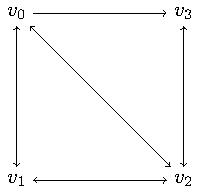
\includegraphics[scale=1]{figures/ExampleGraph.pdf}
\caption{Example Graph}
\end{figure}

For example the bitstring $11,00,01,10$ would be translated to $3-0-1-2$. This means $v_0$ is on the position $3$, $v_1$ in on the position $0$ and so on. The resulting cycle is $(v_1, v_2, v_3, v_0)$.
The search space includes every possible permutation of the positions of the vertices in the hamiltonian cycle. Therefore, its size is $2^{N\log n} = N^N$. The solutions of the HC problem satisfy two conditions:
\begin{enumerate}
\item Each vertex should have a different position.
\item Vertices with consecutive positions have to be connected by an edge. (The last and first positions are considered adjacent)
\end{enumerate}
\begin{table}[htbp]
    \centering
    \begin{tabular}{|c|c|c|c|}
        \hline
        Bitstring & Integer representation & Validity & Cycle \\
        \hline
        00,01,10,01 & 0-1-2-1 & Violates constraint 1 & None \\
        01,11,10,00 & 1-3-2-0 & Violates constraint 2 & $(v_3, v_0, v_2, v_1)$ \\
        00,11,10,01 & 0-3-2-1 & Yes & $(v_0, v_3, v_2, v_1)$\\
        \hline
    \end{tabular}
    \label{tab:example}
    \caption{Some examples of the possible solution encodings.}
\end{table}

An algorithm to solve the HCP of a directed graph with $N = 2^n$ vertices is presented. The main contribution of this paper is the oracle $O$ that flips the phase of the states that satisfy both constraints. Later, possible adaptations of the algorithm for arbitrary graphs are proposed.

\subsection{Circuit initialization}
The position index register $\ket{\psi}$, which covers the search space, has $m = N\log N$ qubits. Applying $O$ requires the addition of two registers, one for each constraint. An ancilla register $\ket{\theta}$ of $k = C^N_2$ qubits, and a second ancilla register $\ket{\zeta}$ with $l$ qubits. $l$ is the number of edges of the  complementary graph.\\
Firstly, all position index qubits should be set in superposition of all states in the search space. This is done by applying the Hadamard Gate to each qubit in the main register. The qubits in the ancillas are set to $\ket{1}$ with the NOT gate. The resulting state is expressed as:
$$\ket{\psi_0} \otimes \ket{\theta_0} \otimes \ket{\zeta_0}$$
where:
$$\ket{\psi_0} = \frac{1}{\sqrt{2^m}}\sum_{i=0}^{m} \ket{i}$$
$$\ket{\theta_0} = \ket{1}^{\otimes k}$$
$$\ket{\zeta_0} = \ket{1}^{\otimes l}$$

\subsection{Grover's Operator}
The Grover operator is composed of two parts, the oracle $O$ and the diffusion operator $D$. The oracle is the main contribution of this paper, and it is divided into three blocks: Positional Exclusivity, Missing Edge Detector, and a multi-controlled phase shift. The diffusion operator is the same as in the original Grover's algorithm.
\subsubsection*{Positional Exclusivity Block}
To satisfy the first constraint, the position of each vertex is compared with the position of every other vertex. The comparison is made by a comparator circuit defined in \cite{Coloring1}. The circuit, composed of NOT, CNOT and Toffoli/MCT gates, is applied to two registers of the same size, $a$ and $b$, and  stores the result in an ancilla qubit $o$.
$$\text{Comparator}(a, b, o) =
\begin{cases}
o \oplus 1, & \text{if } a = b; \\
o, & \text{if } a \neq b.
\end{cases}$$
\begin{figure}[hbtp]
\centering
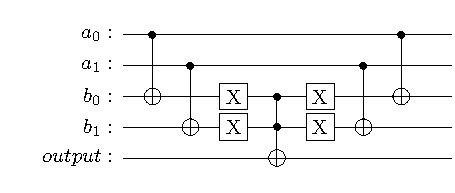
\includegraphics[scale=0.5]{figures/comparator.pdf}
\caption{Two bits Comparator circuit}
\end{figure}

The comparator circuit is applied to the $C^N_2$ combinations of position indexes, and each result is stored in a different qubit of $\ket{\theta}$ If any two vertices are assigned the same position, at least one qubit in $\ket{\theta}$ will be in state $\ket{0}$.

\begin{figure}[hbtp]
\centering
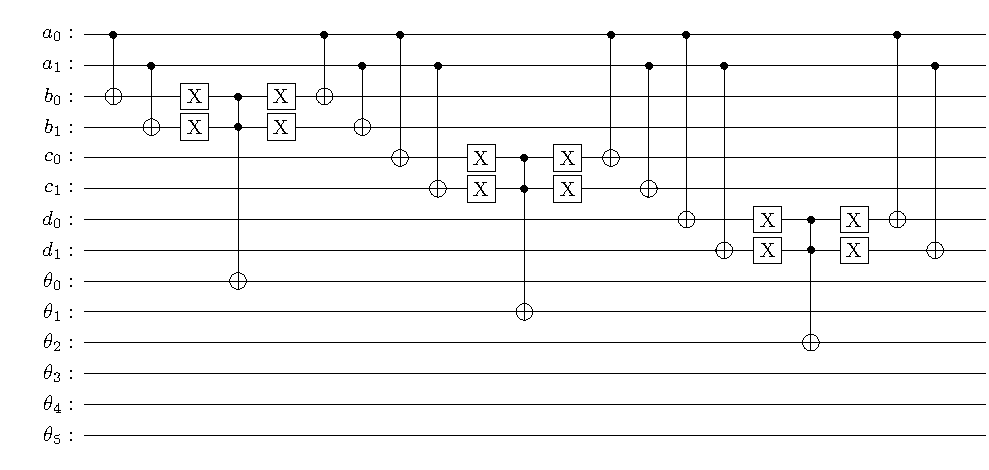
\includegraphics[scale=0.5]{figures/comparator_extended.pdf}
\caption{First three comparisons in the Positional Exclusivity block of the example above.}
\end{figure}

\subsubsection*{Missing Edge Detector Block}

Another subcircuit is introduced in this part, called the Plus One circuit. This circuit takes state $\ket{i}$ to state $\ket{(i+1) \mod 2^p}$. Given a register $q$ with $p$ qubits, a MCT is applied with the $p-1$ least significant qubits as control, and the most significant qubit as the target. This process is repeated taking with the $p-1$ least significant bits, so that every step the MCT has one less control. The inverse circuit, named Minus One circuit, takes state $\ket{i}$ to state $\ket{(i-1) \mod 2^p}$.
\begin{figure}[hbtp]
\centering
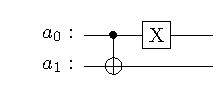
\includegraphics[scale=1]{figures/plus_one.pdf}
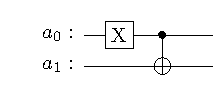
\includegraphics[scale=1]{figures/minus_one.pdf}
\caption{2 qubits Plus One circuit and Minus One Circuit}
\end{figure}

The missing edges set is defined as the set of edges of the complementary graph. In the example, the set of missing edges is $\{(1,3),(3,1),(3,0)\}$. To satisfy the second constraint, the vertices on adjacent positions should not have a missing edge between them.\\
The Plus One circuit is used to take the vertex to the next position, and then the Comparator circuit is used on the vertexes of the missing edge. If the next position of the vertex is occupied by a vertex that has a missing edge between them, the Comparator will flip an ancilla qubit.
\begin{figure}[hbtp]
\centering
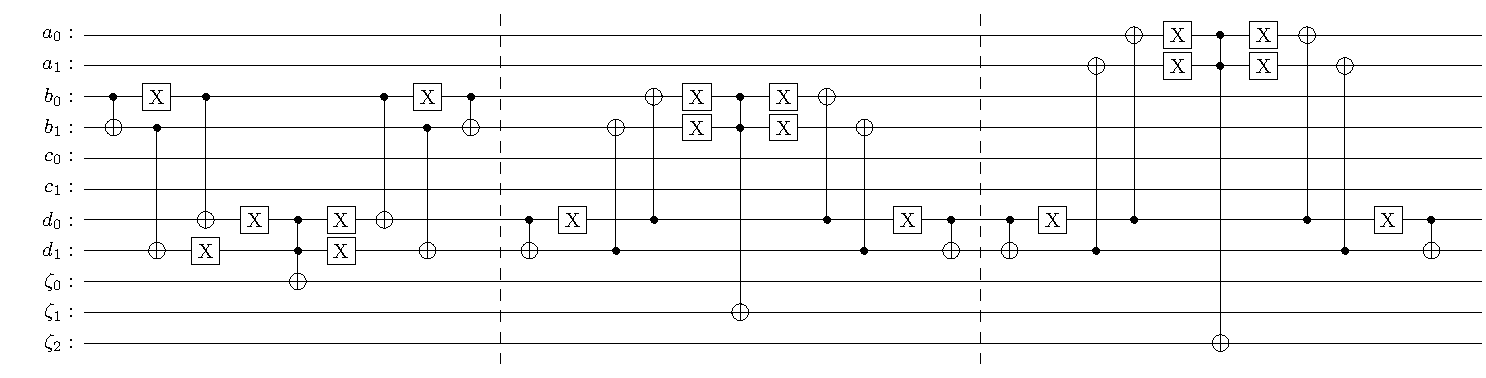
\includegraphics[scale=0.5]{figures/missing_edge.pdf}
\caption{Missing Edge block of the example above}
\end{figure}

\subsubsection*{Complete Oracle Structure}
The complete oracle consists of the Positional Exclusivity Block, a Missing Edge Block, and a multi-controlled phase shift, acting in all the ancilla qubits. Then, the Positional Exclusivity Block and the Missing Edge Block are repeated to return the ancillas to their original state.

\begin{figure}[hbtp]
\caption{Oracle}
\centering
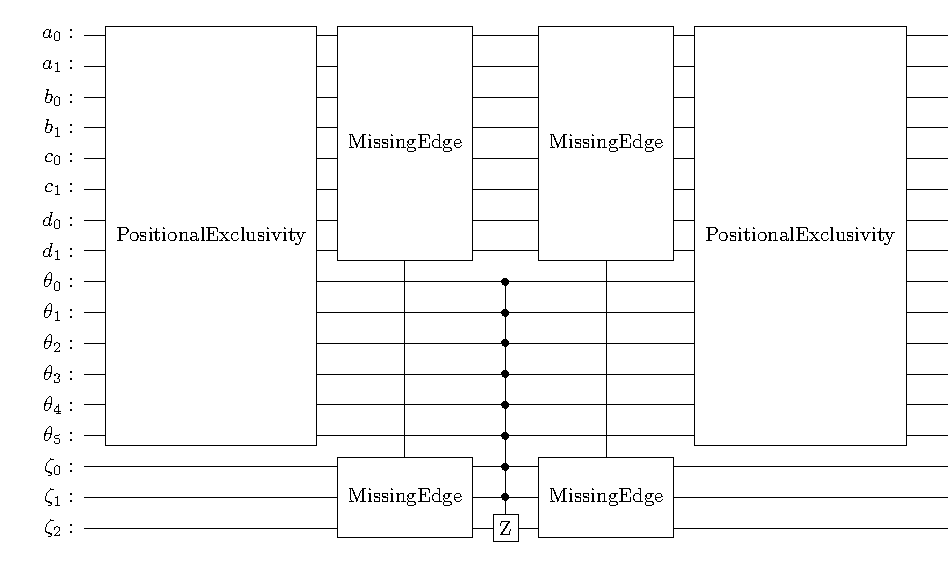
\includegraphics[scale=0.6]{figures/oracle.pdf}
\end{figure}

\subsubsection*{Diffusion Operator}

The diffusion operator is applied on the position\_index register.

\section{Ancilla Reutilization}
This approach employs a distinct ancilla register for each constraint enforcement. It is possible to reuse the ancilla, which helps minimize the required qubit count. Moreover, it reduces the size of the maximum MCT gate needed. However, this strategy involves a tradeoff between qubit quantity, circuit length, and gate utilization. This tradeoff is studied in \cite{SAT_paralel}.\\
A second oracle that employs a single ancilla register is proposed.
\subsection{Circuit description}
The position\_index register $\ket{\psi}$ and $\ket{\theta}$ remain the same, but the $\ket{\zeta}$ register is reduced to a single qubit, initializated in the $\ket{0}$ state.\\
It is important for this formulation that the maximum amount of qubits needed for the missing edge block is less than $C^N_2$. The maximum number of edges a directed graph can have is $2C^N_2$. However, if both edges $(u, v)$ and $(v, u)$ are missing, the same ancilla can store the result of the comparison. This is because a vertex can not have the previous and the next position of another vertex in any cycle of more than two elements. Therefore, the constraints are exclusionary, and a single qubit can be used as a witness for both.\\
The proposed oracle follows these steps: it initiates with the ME block and applies an MCT controlled by the $\ket{\theta}$ with $\ket{\zeta}$ as the target, another ME block is used to return the ancilla register to its initial state. Subsequently, the PE block is executed. The ancilla registers will be in state $\ket{1}$ for valid solutions, therefore, a phase shift is applied on $\ket{\zeta}$ controlled by $\ket{\theta}$. The inverse circuit is applied in order to restore the ancilla to its initial state.\\
An analysis of the circuit with a diagram of its structure is given in Appendix A.

\section{Generalization for an arbitrary graph}

Adapting the oracle for a graph with an arbitrary number of vertices faces two challenges. Firstly, the superposition of states introduces invalid positions, where it is nonsensical for a vertex to occupy, for instance, the 15th position in a cycle of 10 elements. To address this issue, a strategy akin to the one employed in \cite{Coloring1} can be applied, introducing an invalid position block.\\
The second challenge is associated with the Plus One circuit. This circuit efficiently transitions a state from $\ket{i}$ to $\ket{(i + 1) \mod 2^p}$. However, constructing a circuit to transition a state from $\ket{i}$ to $\ket{(i + 1) \mod l}$ for an arbitrary $l$ is more intricate. A modular adder is proposed in \cite{modular}, using additional ancilla registers.\\
The alternative approach followed is to seek a transformation that transforms graphs with an arbitrary number of vertices into graphs with a number of vertices that is a power of two. This transformation should maintain the existing Hamiltonian cycles without introducing new ones.\\
The selected transformation operates as follows: for an arbitrary vertex, it is split into a set of connected vertices. The first vertex of the set retains all the edges that entered the original vertex, while the last vertex preserves all the edges that exited the original vertex. Mathematically, let $G = (V, E)$ represent the original graph, where $V = \{v_1, v_2, ..., v_n\}$ is the set of vertices and $E$ is the set of edges. The transformation $T : (V, E) \rightarrow (V\prime, E\prime)$ transforms vertex $v_n$ in $V$ into $(2^{\lceil \log_2{n} \rceil} + 1 -n)$ vertices $U = \{u_{in}, u_{1}, u_{2}, \dots, u_{out}\}$. . $G\prime = (V\prime, E\prime)$ is defined as follows:
$$V' = \{v_1, v_2, \dots, v_{n-1}\} \cup U$$
$$ E' = \{(v'_j, v'_i) \hspace{5pt} | \hspace{5pt} (v_j, v_i) \in E, \text{ where } i \neq n \text{ and } j \neq n\} $$
$$\cup \{(v'_j, u_{in}) \hspace{5pt} | \hspace{5pt} (v_j, v_n) \in E\} $$
$$\cup \{(u_{out}, v'_j) \hspace{5pt}|\hspace{5pt} (v_n, v_j) \in E\} $$
$$\cup \{(v_i, v_j) \hspace{5pt} | \hspace{5pt} v_i, v_j \in U\}$$

Fig. 9 and Fig. 10 show the transformation for two example graphs.

\begin{figure}[hbtp]
\centering
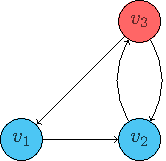
\includegraphics[scale=1]{figures/three_graph.pdf}
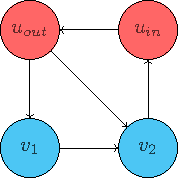
\includegraphics[scale=1]{figures/three_to_four.pdf}
\caption{Transformation from a 3-node graph to a 4-node graph}
\end{figure}

\begin{figure}[hbtp]
\centering
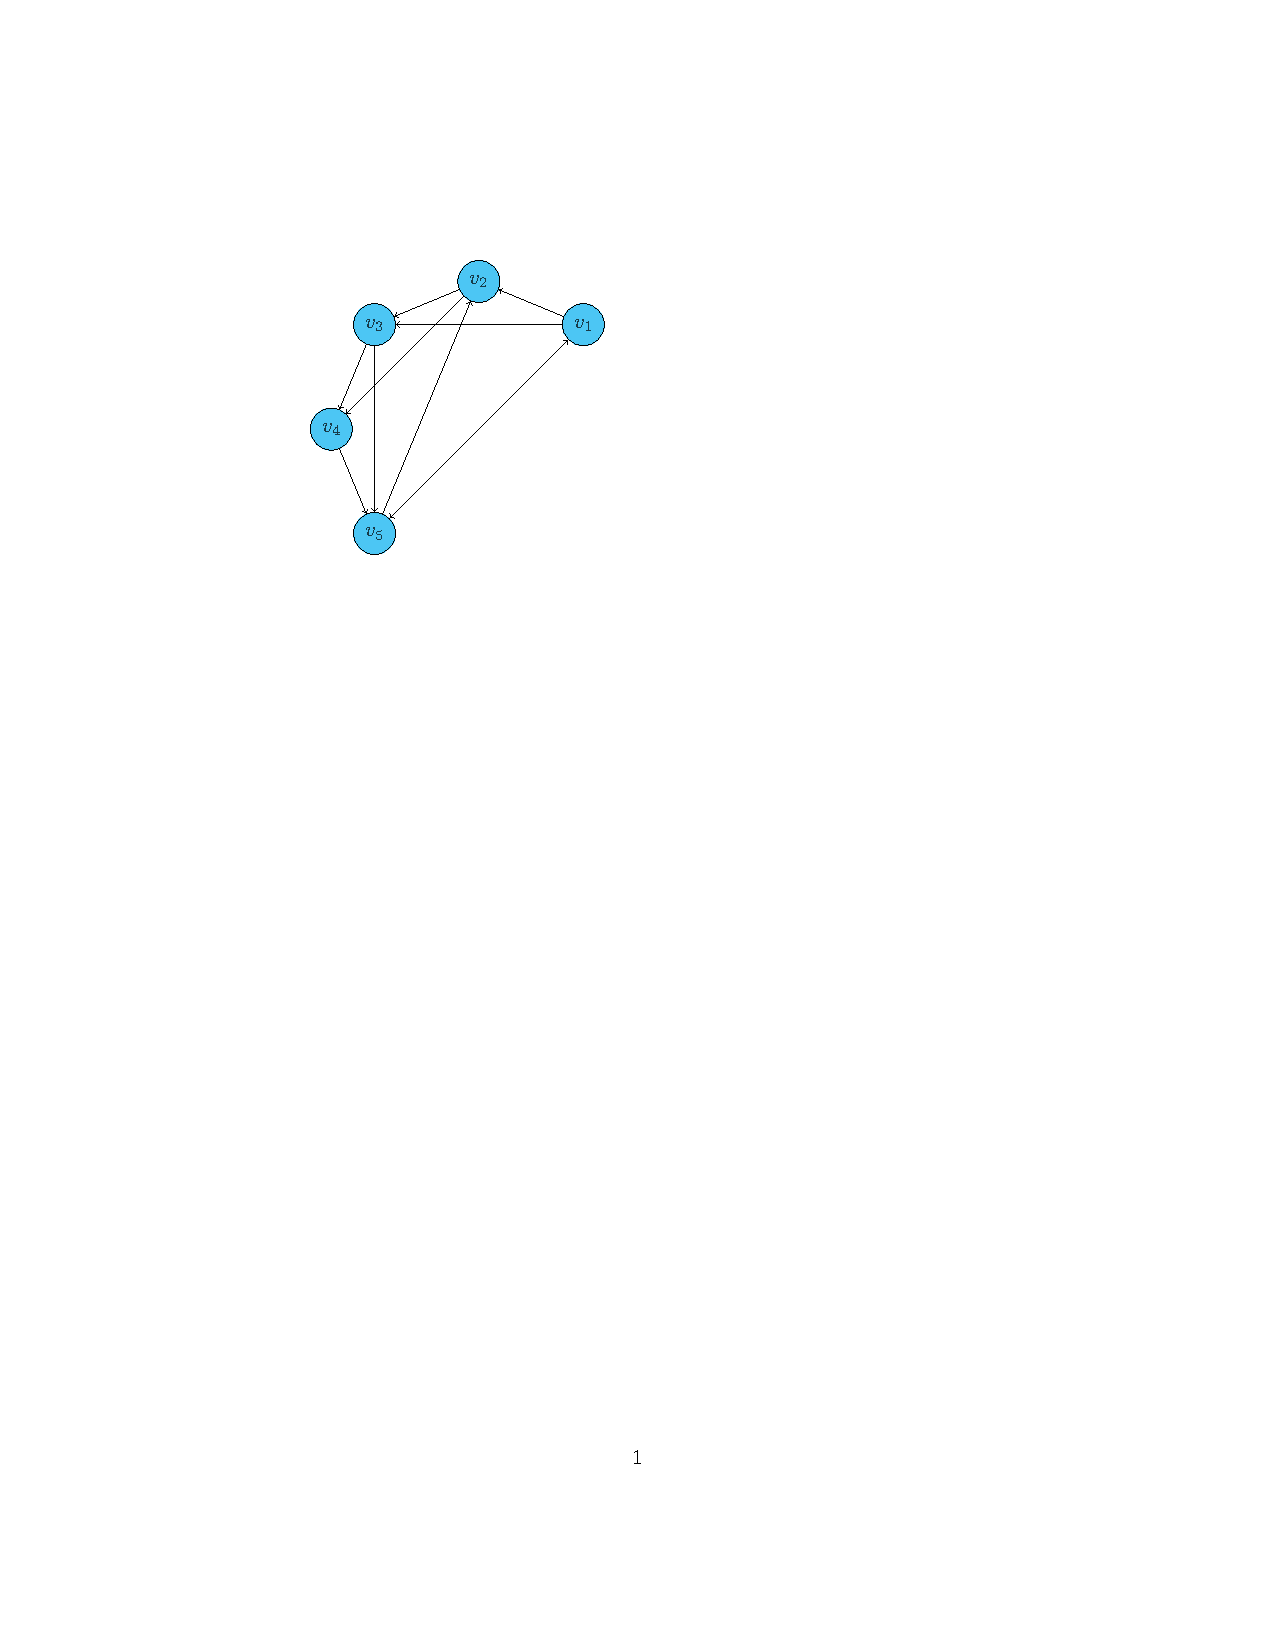
\includegraphics[scale=0.9]{figures/five_graph.pdf}
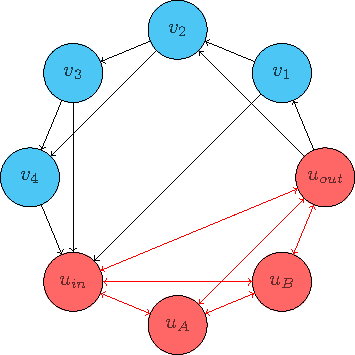
\includegraphics[scale=0.78]{figures/five_to_eight.pdf}
\caption{Transformation from a 3-node graph to a 4-node graph}
\end{figure}


\section{Discussion}
A main challenge in the implementation of the proposed algorithm is determining $k_{Gr}$ when the number of solutions is not known. \cite{Nielsen_Chuang_2010} propose an algorithm that combines the Grover operator with the phase estimation technique to estimate the number of solutions. This algorithm requires the implementation of a Quantum Fourier Transform, which is a complex circuit.\\
Another approach is to choose a fixed $k_{Gr}$ and run the algorithm multiple times. The probability of finding the solution increases with the number of runs. If there is no solution for the problem, the solution distribution will be uniform, with no solution having a greater probability than the others. If there are solutions, the valid states will be amplified.\\
This algorithm is quadratic in the number of vertices $n$. The first formulation uses at most $n\log{n} + 2 n(n-1)/2$ qubits, while the second formulation uses a fixed number of qubits $n \log{n} + n(n-1)/2 + 1$. Both formulations require $O(n^2)$ gates for the oracle, that should be applied $k_{Gr}\approx \sqrt{n^n}$ times. Therefore, the order of the algorithm is $O(n^2 2^{\frac{n \log n}{2}})$.\\
Asymptotically, the quantum algorithm requires the square root of the number of operation a brute force classical algorithm requires. Checking the $n!$ permutations results in an algorithm of order $O(n^2 2^{n \log n})$ \cite{quantum_hamiltonian}.\\
Some examples of the algorithm running on a simulator are shown in Fig. 9. The algorithm was implemented in Qiskit \cite{Qiskit}, and the results were obtained by running the algorithm on a classical simulator. The algorithm was run with $n = 4$ vertices.
The results are presented for each graph with one iteration of the oracle and with the optimum number of iterations of the Grover operator. The histogram of results for each run is presented with 1000 shots. The results show that the algorithm converges to the correct solution with high probability when using the optimum $k_{Gr}$.\\ 

\begin{figure}[hbtp]
\centering
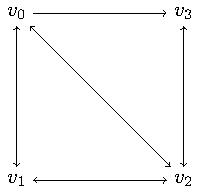
\includegraphics[scale=1]{results/example_1_graph.pdf}
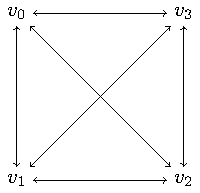
\includegraphics[scale=1]{results/example_2_graph.pdf}
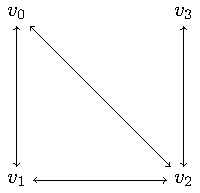
\includegraphics[scale=1]{results/example_3_graph.pdf}
\caption{Graphs used as test cases for the algorithm}
\end{figure}

%Example with 1 and 8 iterations
\begin{figure}[hbtp]
\centering
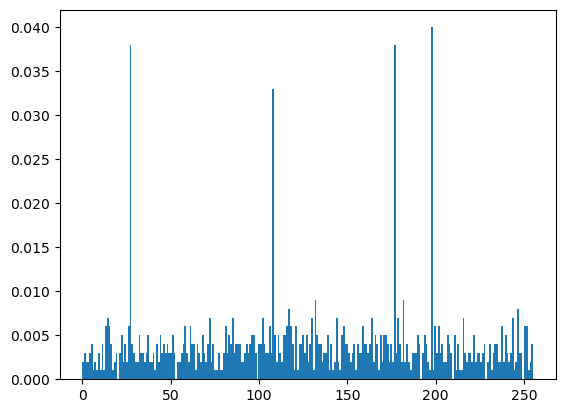
\includegraphics[scale=0.5]{results/example_1_1_iteration.png}
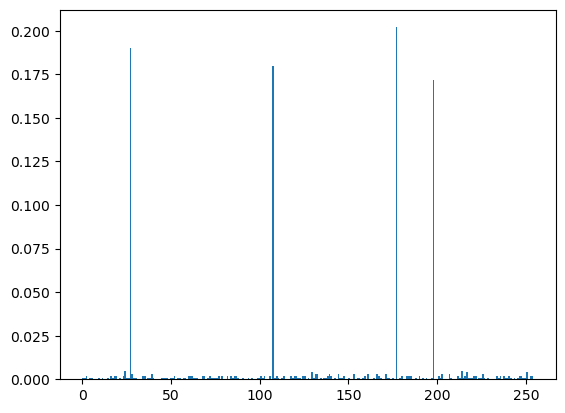
\includegraphics[scale=0.5]{results/example_1_8_iterations.png}
\caption{Examples of the graphs of the algorithm running on a simulator}
\end{figure}
% Example with 1 and 2 iterations
\begin{figure}[hbtp]
\centering
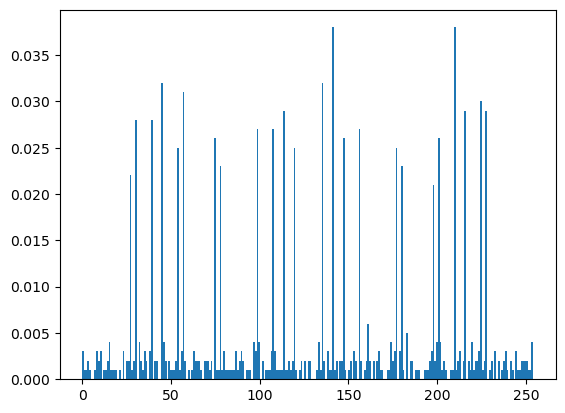
\includegraphics[scale=0.5]{results/example_2_1_iteration.png}
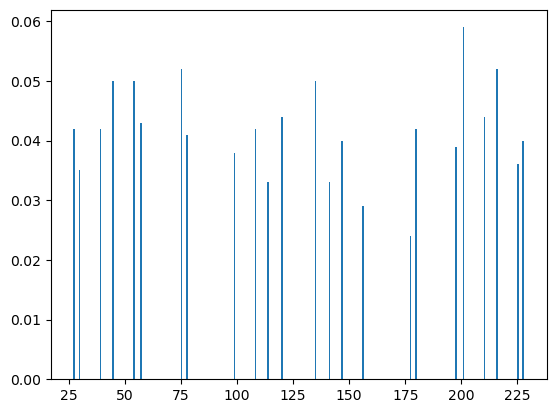
\includegraphics[scale=0.5]{results/example_2_2_iterations.png}
\caption{Examples of the graphs of the algorithm running on a simulator}
\end{figure}

\begin{figure}[hbtp]
\centering
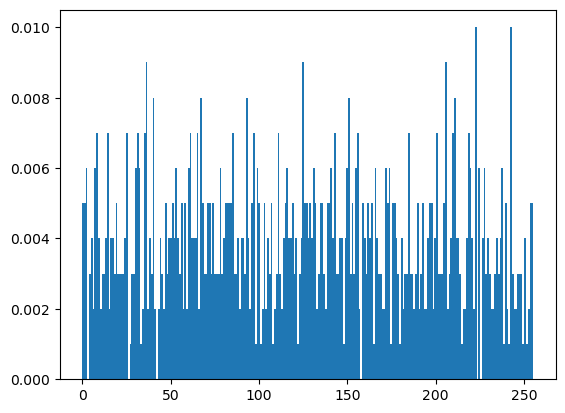
\includegraphics[scale=0.5]{results/example_3.png}
\caption {Example of the graph of the algorithm running on a simulator}
\end{figure}

\section{Conclusion}
In this paper, we have proposed a quantum algorithm to solve the Hamiltonian Cycle Problem using Grover's algorithm. The algorithm presents a quadratic advantage over brute force classical algorithms. The algorithm was implemented in Qiskit and tested on a classical simulator. The algorithm was implemented with two different formulations of the oracle, one that uses a distinct ancilla register for each constraint and another that reuses the ancilla register. The second formulation reduces the number of qubits needed, but it requires a fixed number of qubits. The algorithm was tested on graphs with 4 vertices, and the results show that the algorithm converges to the correct solution with high probability.\\
Present heuristic algorithms are successful in solving the problem for many instances, but they are not guaranteed to find the optimal solution. The proposed algorithm offers a quadratic speedup over classical algorithms, and it is a promising approach to solve the Hamiltonian Cycle Problem.\\

\bibliography{references.bib} 
\bibliographystyle{ieeetr}

\section*{Appendix A: Circuit Analysis of the second oracle}
Fig. 8 shows the diagram of the complete oracle $O$. The first generic run of the oracle will be analyzed. The solution space is divided into four groups. The $A$ states that represent a valid hamiltonian cycle $\alpha$,the $B$ states that only satisfy the missing edge constraint $\beta$, the $C$ states that only satisfy the positional exclusivity constraint $\gamma$, and the rest of the $D$ states $\delta$.

$$
\ket{\rho_0} = \frac{1}{2^m} \left( \sum_{i=1}^{A} \ket{\alpha_i} + \sum_{i=1}^{B} \ket{\beta_i} + \sum_{i=1}^{C} \ket{\gamma_i} + \sum_{i=1}^{D} \ket{\delta_i} \right) \otimes \ket{1}^{\otimes k} \otimes \ket{0}
$$

In $\ket{\rho_1}$, the ancilla of the states $C$ and $D$ have at least one flipped qubit. The string of $k$ qubits that are not all in state $\ket{1}$ will be represented with a $\ket{l}$.

$$
\ket{\rho_1} = \frac{1}{2^m} \left( \sum_{i=1}^{A} \ket{\alpha_i} \ket{1}^{\otimes k} + \sum_{i=1}^{B} \ket{\beta_i} \ket{1}^{\otimes k} + \sum_{i=1}^{C} \ket{\gamma_i} \ket{l_{\gamma_i}} + \sum_{i=1}^{D} \ket{\delta_i} \ket{l_{\delta_i}} \right) \otimes \ket{0}
$$

The $\ket{\zeta}$ state is only flipped for the states that have the $\ket{\theta}$ ancilla in state $\ket{1}^{\otimes k}$.

$$
\ket{\rho_2} = \frac{1}{2^m} \left( \sum_{i=1}^{A} \ket{\alpha_i} \ket{1}^{\otimes k} \ket{1} + \sum_{i=1}^{B} \ket{\beta_i} \ket{1}^{\otimes k} \ket{1} + \sum_{i=1}^{C} \ket{\gamma_i} \ket{l_{\gamma_i}} \ket{0} + \sum_{i=1}^{D} \ket{\delta_i} \ket{l_{\delta_i}} \ket{0} \right)
$$

The second missing edge block returns the ancilla to its initial state.

$$
\ket{\rho_3} = \frac{1}{2^m} \left( \sum_{i=1}^{A} \ket{\alpha_i} \ket{1}^{\otimes k} \ket{1} + \sum_{i=1}^{B} \ket{\beta_i} \ket{l_{\beta_i}} \ket{1} + \sum_{i=1}^{C} \ket{\gamma_i} \ket{1}^{\otimes k} \ket{0} + \sum_{i=1}^{D} \ket{\delta_i} \ket{1}^{\otimes k} \ket{0} \right)
$$

The positional exclusivity block changes the ancilla of states $\ket{\beta}$ and $\ket{\delta}$.

$$
\ket{\rho_4} = \frac{1}{2^m} \left( \sum_{i=1}^{A} \ket{\alpha_i} \ket{1}^{\otimes k} \ket{1} + \sum_{i=1}^{B} \ket{\beta_i} \ket{l_{\beta_i}} \ket{1} + \sum_{i=1}^{C} \ket{\gamma_i} \ket{1}^{\otimes k} \ket{0} + \sum_{i=1}^{D} \ket{\delta_i} \ket{l_{\delta_{2i}}} \ket{0} \right)
$$

In state $\ket{\rho_5}$, the $\ket{\alpha}$ states are flipped.

$$
\ket{\rho_5} = \frac{1}{2^m} \left( \sum_{i=1}^{A} \ket{\alpha_i} \ket{1}^{\otimes k} \ket{1} + \sum_{i=1}^{B} \ket{\beta_i} \ket{l_{\beta_i}} \ket{1} + \sum_{i=1}^{C} \ket{\gamma_i} \ket{1}^{\otimes k} \ket{0} + \sum_{i=1}^{D} \ket{\delta_i} \ket{l_{\delta_{2i}}} \ket{0} \right)
$$

The next blocks return the ancilla registers $\ket{\theta}$, $\ket{\zeta}$, and $\ket{\psi}$ to their initial states.

$$
\ket{\rho_8} = \frac{1}{2^m} \left( - \sum_{i=1}^{A} \ket{\alpha_i} + \sum_{i=1}^{B} \ket{\beta_i} + \sum_{i=1}^{C} \ket{\gamma_i} + \sum_{i=1}^{D} \ket{\delta_i} \right) \otimes \ket{1}^{\otimes k} \otimes \ket{0}
$$

\begin{figure}[hbtp]
\centering
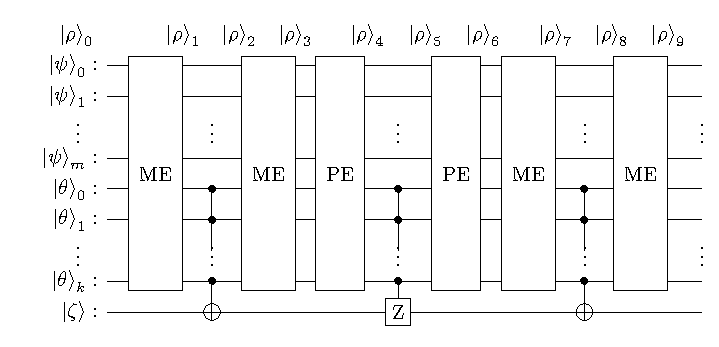
\includegraphics[scale=0.8]{figures/oracle_circuit.pdf}
\caption{Oracle with ancilla reutilization}
\end{figure}
\end{document}
